
\section{学生処分問題と熊野寮自治会の対応}
\label{sec:shobun}
\bunsekisha{文責}{対処分戦略推進局}
\index{がくせいしょぶん@学生処分|textbf}


高校でも生徒が「問題」行動を起こした時に、反省文を書かされたり、停学にさせられるなどの処分が行われることがありますが、京大でも似たような措置が不当かつ恣意的に行われ、学生の自由と人権が抑圧されているという現状があります。近年の京大では吉田寮問題や立て看問題(後述)など、大学当局からの学生への抑圧が強まっており、徐々に自由な雰囲気を失いつつあります。しかし京大には、今の自由を守ろう、いや、今よりもっと自由な京大を作ろう、と考え行動している学生がまだまだたくさんいます\index{じゆうのがくふう@自由の学風}。処分はそうした「問題」行動を起こす学生への脅しとして使われてしまっているのです。ここでは、熊野寮の要求書提出時に職員に抗議した3名の寮生が無期停学処分にされたこと、京大の二次試験の会場に像を設置した寮生1名が\ruby{譴責}{けん|せき}処分にされたこと、時計台占拠というイベントに参加したとして8名の学生が処分されたことの3つの事例を紹介し、何が問題なのか、今まで寮としてどんな対応をしてきたか、これからどうするべきか、ということについて書きたいと思います。

\begin{shadebox}
{\large\textbf{出る順! 処分問題単語帳}}
\begin{description}
    \item[処分(正式には「学生懲戒処分」)] 当局が「問題だ」と考える学生に当局が与える罰。京都大学学生懲戒規定(\url{https://www.kyoto-u.ac.jp/uni_int/kitei/reiki_honbun/w002RG00000283.html})に手続きの定めがある。要は、当局の都合の悪い学生を屈服されるための最終手段。 処分の軽重は学部の教授会が上申するが、最終的には当局が決定する。
    \item[当局(「大学当局」「京大当局」とも)] 法律上京都大学で一番偉い「役員会」(「理事会」と言われることも多い)を中心とした大学執行部やその意向を受けて学生と対峙することになる職員全般を指す。単に「京大」とか「京都大学」だと、教授会のことを指すのか、役員会のことを指すのか、僕ら学生のことを指すのか、それともそうしたものを全部ひっくるめているのか、分からないので「当局」は便利な言葉だ。処分問題に限らず京大内では頻出語なので絶対に憶えておこう。\index{だいがくとうきょく@大学当局}
    \item[教授会] 	各学部(学科)の教員で構成される会議体で、昔はとっても偉くて学部ごとの独立が強かった(学部自治)けど、今は役員会の方が偉くなってしまった。
    \item[学生自治会] 学部や寮などに組織されている学生全員加盟制の自治会。学生のために自分たちで動いたり、当局と交渉したりしている。学生自治会がない学部や寮もある。熊野寮自治会は学生自治会の一つだ。\index{がくせいじちかい@学生自治会}
    \item[停学] 大学構内に入れず、当然授業も受けれず、図書館も使えないのに授業料は満額取られてしまうというヒドい処分。有期停学(6月未満)と無期停学がある。無期停学よりヒドい処分としては、京大に在籍したという記録自体が抹消され、学生の身分も剥奪される「放学処分」がある。\index{ていがく@停学}
    \item[\ruby{譴責}{けん|せき}] 学部長に怒られるという処分。停学よりは軽いが、実質的には「次やれば停学」を言い渡されるようなもので学生の威圧には十分だ。
\end{description}
\end{shadebox}


\subsection{寮生に暴行を振るう職員に抗議しただけで無期停学!?}
熊野寮自治会は自治会として大学当局に要求することを要求書\index{ようきゅうしょ@要求書}にまとめて、当局の「厚生課」と呼ばれる窓口に提出することあります。事件が起こったのは2018年10月の要求書提出のときです。一人の寮生(以下Aとします)が職員に取り囲まれ、暴行を受けました。Aさんが覆面をしていたため、当局はこの行為を「不審者対応」であると称しています。これに対して、提出に参加していた3名の寮生が、職員とAさんの間に割って入り、職員に抗議しました。この抗議が「業務の妨害」とみなされ、2019年9月に3名に対して無期停学処分が下されました。このうち1名はいまだに停学が続いています。


\newpage

\subsection{オルガ像を設置して譴責処分!?}

\begin{wrapfigure}{r}{8zw}
    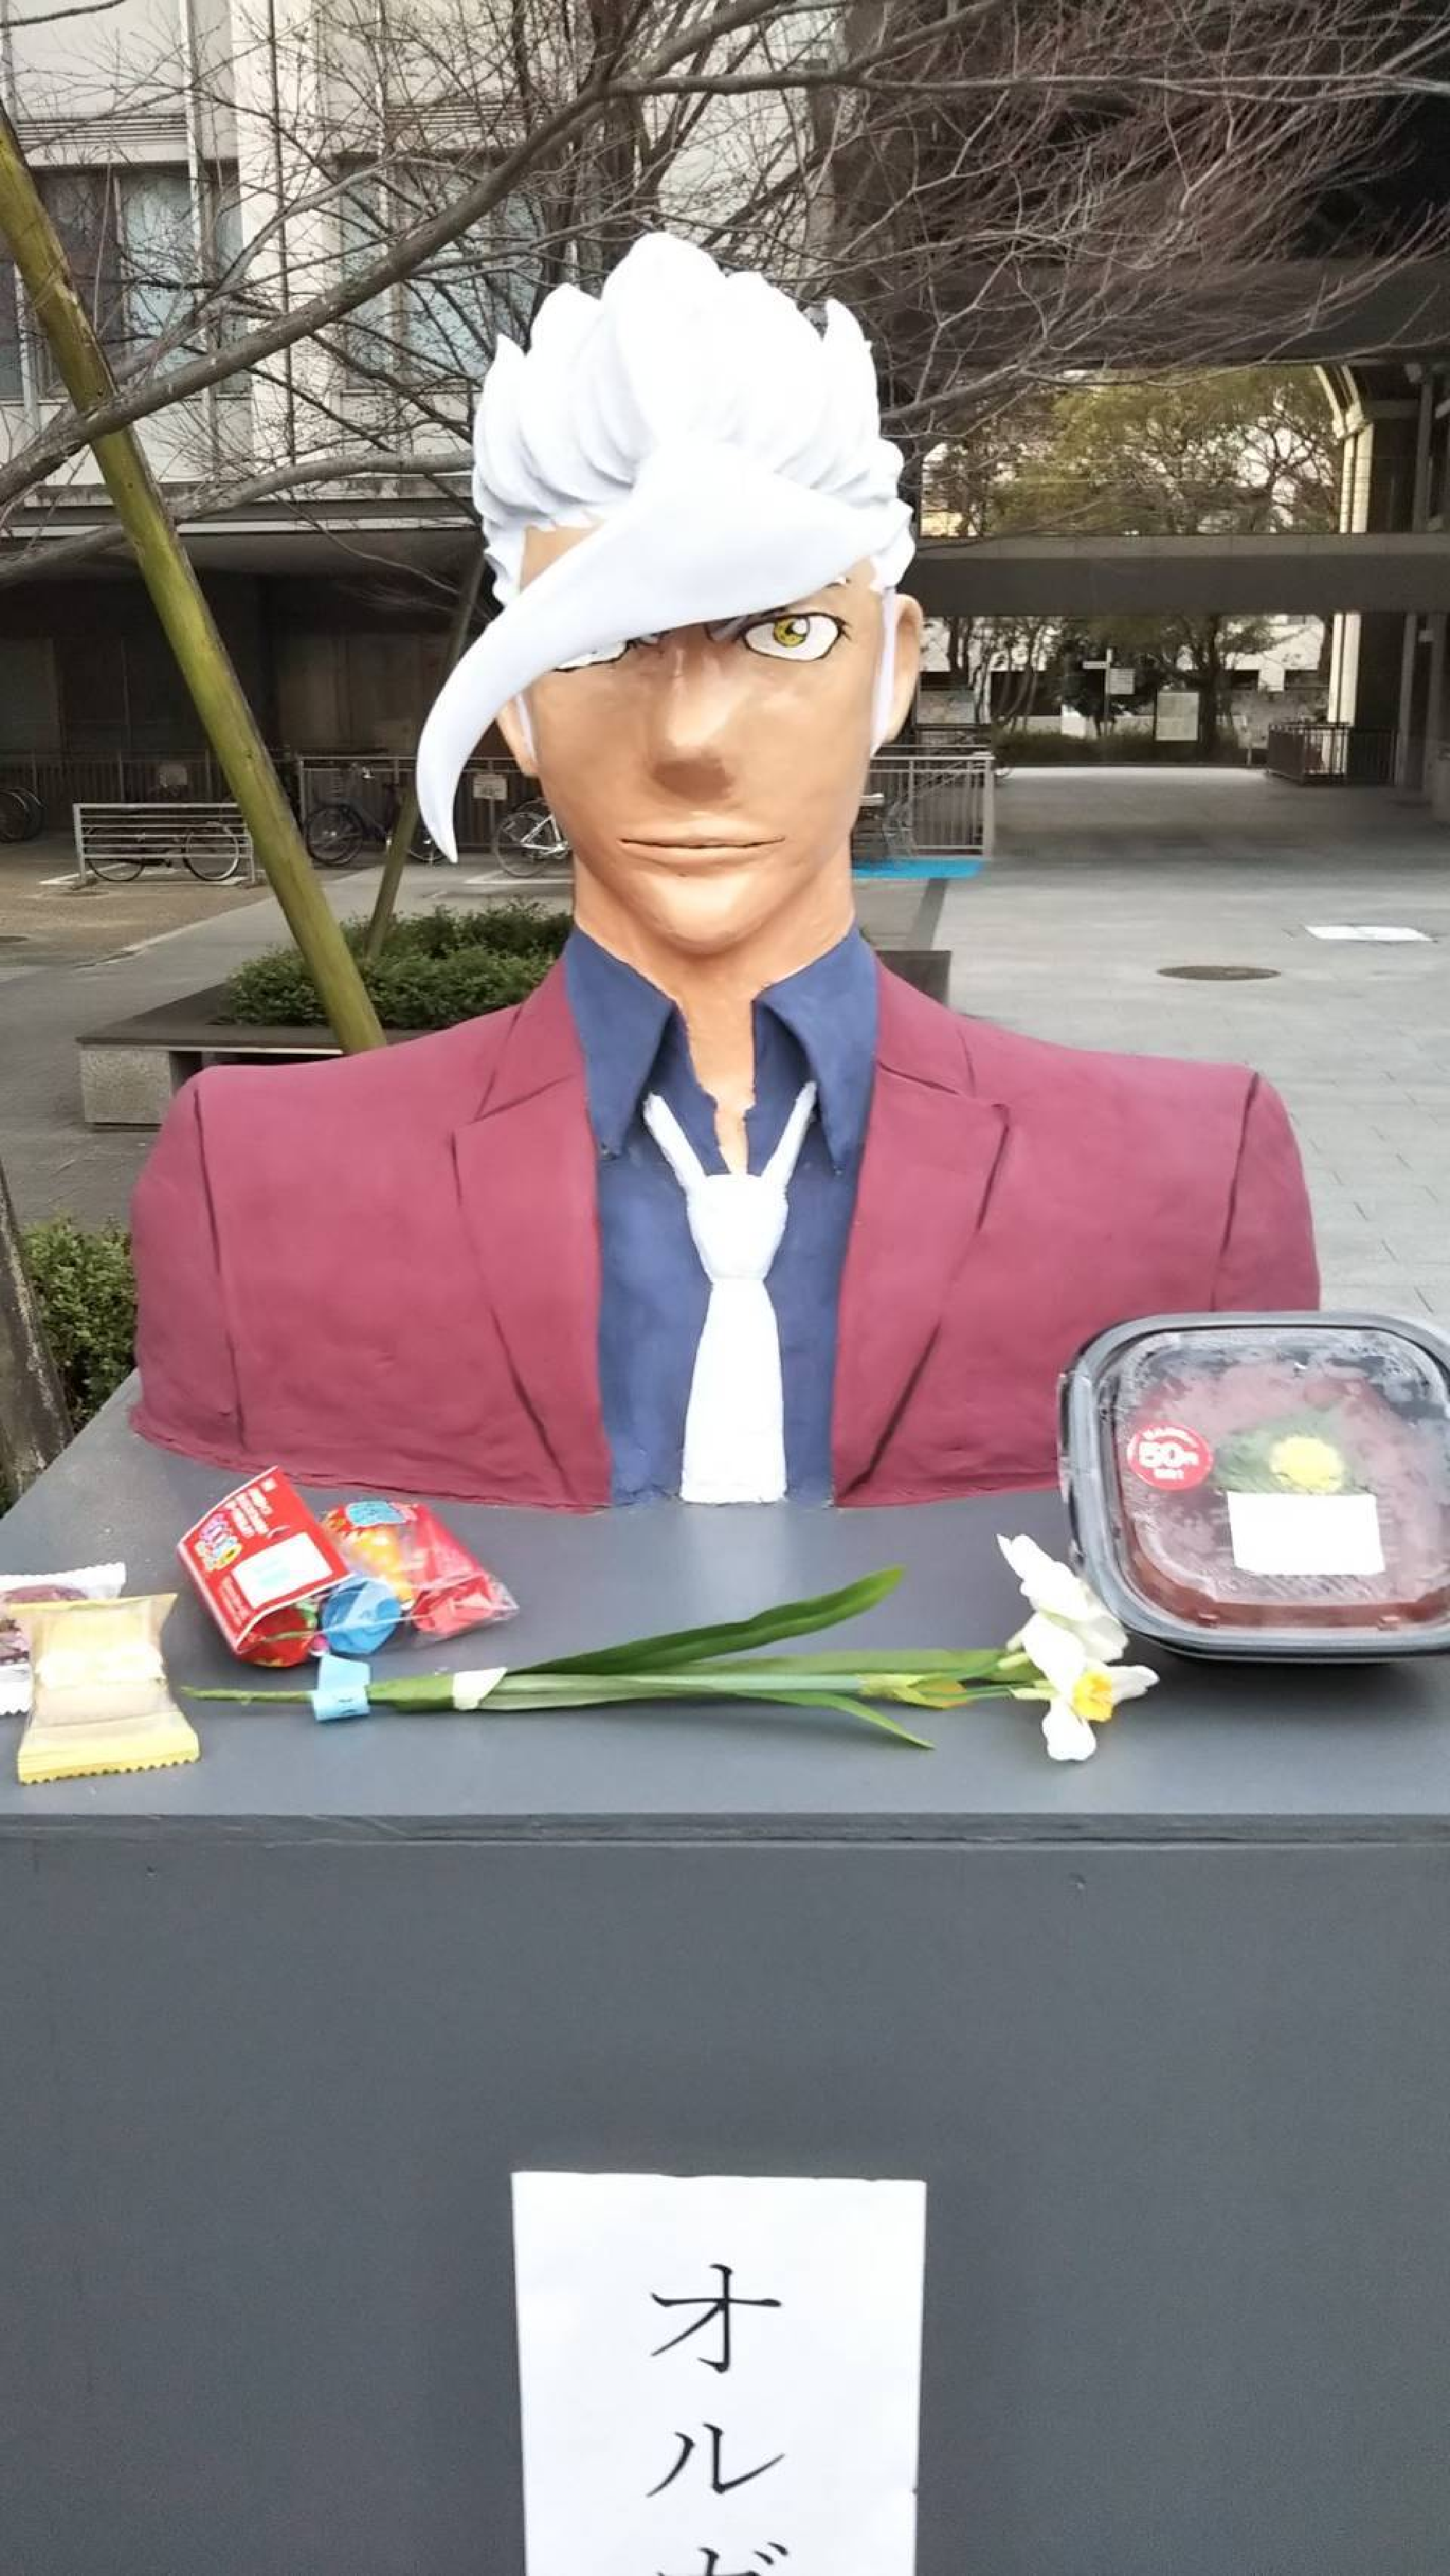
\includegraphics[width=8zw]{gazo/oruga.pdf}
    \captionsetup{labelformat=empty,labelsep=none}
    \caption{オルガ像}
\end{wrapfigure}

\index{おるがぞう@オルガ像}
読んでいる人の多くが京大の二次試験でパンフを受け取ったと思います。京大の二次試験は様々な学生が立て看や像を立てたり、入寮パンフを配ったり、受験生と麻雀をしたりと、構内は受験生激励で非常ににぎやかになります(もちろん試験時間中は静かです)。2019年の入試会場での『機動戦士ガンダム 鉄血のオルフェンズ』のキャラクター「オルガ・イツカ」の像設置も、こうした激励行為の一環として行われました。しかし、この行為が「迷惑行為」「業務の妨害」とみなされ、2020年1月にオルガ像を設置した寮生1名に対して、譴責処分が下りました。

\subsection{時計台に登ろうとして処分!?}
熊野寮祭の恒例企画と言えば「時計台占拠」\index{とけいだいせんきょ@時計台占拠}。京大の時計台に\ruby{梯子}{はし|ご}を掛けて登る企画です。10年以上続いてきた企画で、昔は職員も「危ないからやめなさい」と言いつつ、梯子を支えたり、写真撮影を手伝ったりと安全な企画の貫徹に気を配っていました。しかし、ここ数年は一転し、大勢の職員が梯子を奪ってきたり、掛けられた梯子を揺らしたり、警察を構内に導入して妨害するなど、強固な弾圧に及んでいます。こうした中、2020年に行われた時計台占拠に参加したとして9名の学生に処分に向けた呼び出しがあり、最終的に2021年11月に卒業した1名を除く8名に対し、有期停学や譴責といった処分が下りました。

\subsection{総長室に突入して処分!?}
2022 年の熊野寮祭企画「総長室突入」\index{そうちょうしつとつにゅう@総長室突入}にて学生を扇動し喧騒を激化させたとして、2024年9月に5 人の学生に停学処分が下されました。この企画では、大学を私物化し学生の声を聞こうとしない大学当局、そして総長に対し、団体交渉の再開や学生処分の根拠になっている学内懲戒規程の撤廃などを求める要求書を提出しに行く行動でした。この処分は「喧騒を激化」させたこと、つまり学生が集まって声を上げることそのものを理由とするものです。学生の切実な要求に対して一切回答しないどころか懲戒処分で対応するという、大学当局の不誠実さが明らかになりました。



\subsection{何が問題なの?}
2つの処分の経緯を軽く見ましたが、「処分されて当たり前やん」と思ったかもしれません。しかし、この処分は不当なものです。問題は
\begin{enumerate}
    \item 処分は被処分者の人権を侵害するものである
    \item 被処分者の行為は問題のあるものではない(なのに恣意的に処分規定が適用されている)
    \item 逆に職員の行為こそ問題のあるものだ(なのにそれについては検証されていない)
    \item 処分は学生を威圧し、学生の自由を弾圧するために用いられている
\end{enumerate}
の4つに集約されると思います。一つ一つ説明していきましょう。

\vspace{4mm}
\noindent\fbox{1. 処分は被処分者の人権を侵害するものである}

処分に至るまでの過程、処分内容、処分の解除条件のいずれにおいても学生処分は被処分者の人権を侵害しています。当局の考える「問題」行動を確認された学生には、当該行為について弁明する機会が与えられますが、これには弁護士や第三者を同伴することはできません。呼び出された学生は一人で複数人の教授陣を相手に弁明しなければならず、いわば密室裁判です。また当該学生や学部教授会に証拠が開示されることはありません。つまり無根拠な事実認定が行われているという疑いが拭えないのです(実際に事実に反する、当該学生に不利な認定がなされてきました)。時計台占拠についての処分では、こうした問題性を解決できない限り、呼び出しに応じられないとの旨を、調査を行っていた特別委員会に当該学生が通告しました。それがなければ公正な判断が期待できないからです。しかし、特別委員会は理由なくこの要求を拒否し、処分を強行しました。

被処分者には、処分されたということ自体もそうですし、将来のことや親や友人との関係など精神的に大きな負担がかかります。\index{おや@親!とのかんけい@---との関係}また停学の場合、授業を受けられない、図書館\index{としょかん@図書館}も使えない、構内に入ることさえもできないのに授業料を払わせられ、経済的な負担も大きなものになります。職員に抗議して処分を受けた事例では、自分のやった行為の非を認めなければ停学の解除をしないという良心の自由を侵す条件が当初付けられてもいました\footnote{すでに解除された1名については結局この条件が適用されなかった(後述)。}。これだけの人権侵害をするのならば、被処分者にそれ相応の非がなければならないでしょう。そのような非はあったのでしょうか?

\vspace{4mm}
\noindent\fbox{2. 被処分者の行為は問題のあるものではない}\ \ 
\fbox{3. 逆に職員の行為こそ問題のあるものだ}

要求書提出時に職員に抗議した3名の寮生は、参加者のAさんを職員の暴行から守ろうとしただけであり、これは寮生として普通の行為です。覆面をしていたとはいえ、明らかに熊野寮の提出行動に来ただけの(それも立ち去ろうとしている)Aさんをとっ捕まえ、暴行した職員と比べた時にどれほどの罪があるのかと聞かれれば、首を傾けざるを得ません。オルガ像の事例についても総合人間学部の酒井敏教授の以下のツイート\footnote{\url{https://twitter.com/orita_hikoichi/status/1181407946636267520}と\url{https://twitter.com/orita_hikoichi/status/1181451625442865153}。いずれも2019年10月8日のツイート。}を読むと、被処分者の行為よりもむしろ職員の行動の方がよっぽど「迷惑行為」であり入試「業務の妨害」であったことが分かります。\index{ついったー@ツイッター}

\begin{quotation}
    2019年2月の入試当日のオルガ像が話題になっていますが、現場に最も近い試験会場の入試委員長は私でした。

    オルガ像に関する製作者と大学職員とのやり取りや音楽は全く聞こえず、受験生や試験監督から騒音に関する報告は一切受けていません。もちろん試験の実施に何の支障もありませんでした。

    入試業務では、静かな環境を維持する事が最も重要です。折田先生像やオルガ像の存在そのものは、全く支障はありません。これまで10年以上問題なく存在していたものを、まさに試験時間中に撤去する事は、騒動を引き起こす可能性があり、入試業務に対する重大なリスクです。
\end{quotation}

時計台占拠についても10年以上安全に行われてきました。その企画が危険になったのは職員の強引な妨害が原因です。職員の職務を妨害したことが処分の理由であるのなら、本当にその業務が正当だったのかという検証が必要です。しかし、そのような検証は、処分決定の過程でも処分中においても一切なされないままです。\index{とけいだいせんきょ@時計台占拠}

\vspace{4mm}
\noindent\fbox{4. 処分は学生を威圧し、学生の自由を弾圧するために用いられている}

1,2,3が正しいとすれば、学生の問題のない行為を取り上げて、当局は学生の人権を抑圧していることになりますが、なぜこんなことをするのでしょうか。それは、\textbf{被処分者および他の当局に反抗的な学生を、これ以上反抗的な態度を取らせないように脅すため}です。

近年の京都大学では学生の自由や学生の自治に対する当局からの弾圧が強まっており、学内の自由な雰囲気は徐々に失われています。\index{じゆうのがくふう@自由の学風}例えば1960年代から多くのサークル、政治団体などが立て、名物化していた立て看板\index{たてかん@タテカン}が2017年、京都市の景観条例を理由として、構外に向けたものだけでなく、なぜか構内のものまで規制され、京大とその周辺はすっかり殺風景になってしまいました。また熊野寮と同じく学生自治によって運営されている吉田寮\index{よしだりょう@吉田寮}に、当局から一方的な退去命令が出され、訴訟にまで発展しています\footnote{吉田寮への入寮に関しては、吉田寮の入寮パンフ及び吉田寮ホームページを御覧ください。今年も入寮募集をしています。}。これと前後し、それまで自由に行えていた学内での集会(学生などが休み時間に集まって、アジテーション\index{あじてーしょん@アジテーション}を聞いたり、ビラを配ったり、炊き出しを行ったりする)が職員による妨害や撮影などを受けるようになってしまいました。

上の事例で処分されたのはそうした学生にとっての閉塞状況を打ち破ろうとしていろいろな活動をしていた学生でした。当局は当該の活動への思いを\ruby{挫}{くじ}くために、同じように当局に反抗する学生をこれ以上出さないための見せしめにするために、このような無理やりな狙い撃ち処分を行ったのです。

当局に対して声を上げるという行為ができなくなってきているのは、学生だけではなく教員もそうです。実際、教授会の上申内容よりも重い処分が下された事例も複数ありました。現在の京大はこのように役員会を中心とした独裁国家化しているのです。しかし、京大は役員会のものではないはずです。学生こそ大学の主人公であり、学生の自由な行動こそが京大のこれからを形作っていくべきなのです。


\subsection{熊野寮としての対応}

\begin{wrapfigure}{r}{8zw}
    \vspace*{-8mm}
    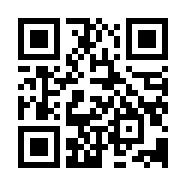
\includegraphics[width=8zw]{gazo/zenshotaishomei.png}
\end{wrapfigure}

熊野寮自治会は2019年から対処分戦略推進局(通称「処分局」)を設けて、毎週会議を行っています。処分局では被処分者と綿密に話し合いながら、不当な処分の撤回・阻止、学生処分という学生全体への攻撃をみんなの力で跳ね返していくことを目的として、処分問題についての広報活動や学内諸団体との連携を行っています。寮生だけでなく、寮外生も参加しています。(毎週火曜日20時から熊野寮食堂で会議してます)

また処分問題を全学的な問題として扱うために、熊野寮自治会処分局、法学部学生自治会処分対策小委員会\index{がくぶじちかい@学部自治会}、全学自治会同学会執行委員会(安田委員長)\index{どうがくかい@同学会}やその他有志によって全学処分対策委員会(全処対)\index{ぜんがくしょぶんたいさくいいんかい@全学処分対策委員会}が2020年3月に結成されています。
熊野寮自治会は直近の処分である総長室突入を理由とした5人の学生に対する停学処分の撤回と、上で述べたように恣意的な運用が可能な学生懲戒規程の撤廃を求める署名を行っています。
右記QRコードまたは\url{https://chng.it/qLmcnQptDc}からぜひ署名お願いします。

寮としてこうした積極的な行動をとるのは、無期停学処分の理由が寮自治会としての要求書提出行動や寮祭企画だったから、というだけではありません。\textbf{一人でも抑圧を受けている学生がいれば、それをみんなの問題として受け止めて行動することが学生自治会の役割だからです}。一人で処分の撤回を訴えても、当局は聞く耳を持たないでしょう。しかし、学生自治会として被処分者と一体となって動き、京大当局に圧力を掛けることができれば、当局は処分の撤回や軽減を考えざるを得なくなるでしょう。また、処分が学生全体を威圧するものとして行われている以上、自治会として積極的に動くことは現在や未来の寮生、学生全体にとっても利益のあることです。先程も言ったように、この処分は京大の自由や学生全体の権利を奪おうとするものです。学生が声を上げる自由がなくなれば、当局が寮を廃止しようとしてきたり、学費を上げようとしてきた場合に、それに反対の声を上げ、学内外での運動を盛り上げることはできません。学内での学生の声を守るために、「不当な学生処分は絶対に許さない」という態度表明が必要です。


\subsection{処分撤回・阻止集会}\index{しょぶんてっかい・そししゅうかい@処分撤回・阻止集会}

\begin{wrapfigure}{r}{18zw}
    \vspace*{-\intextsep}
    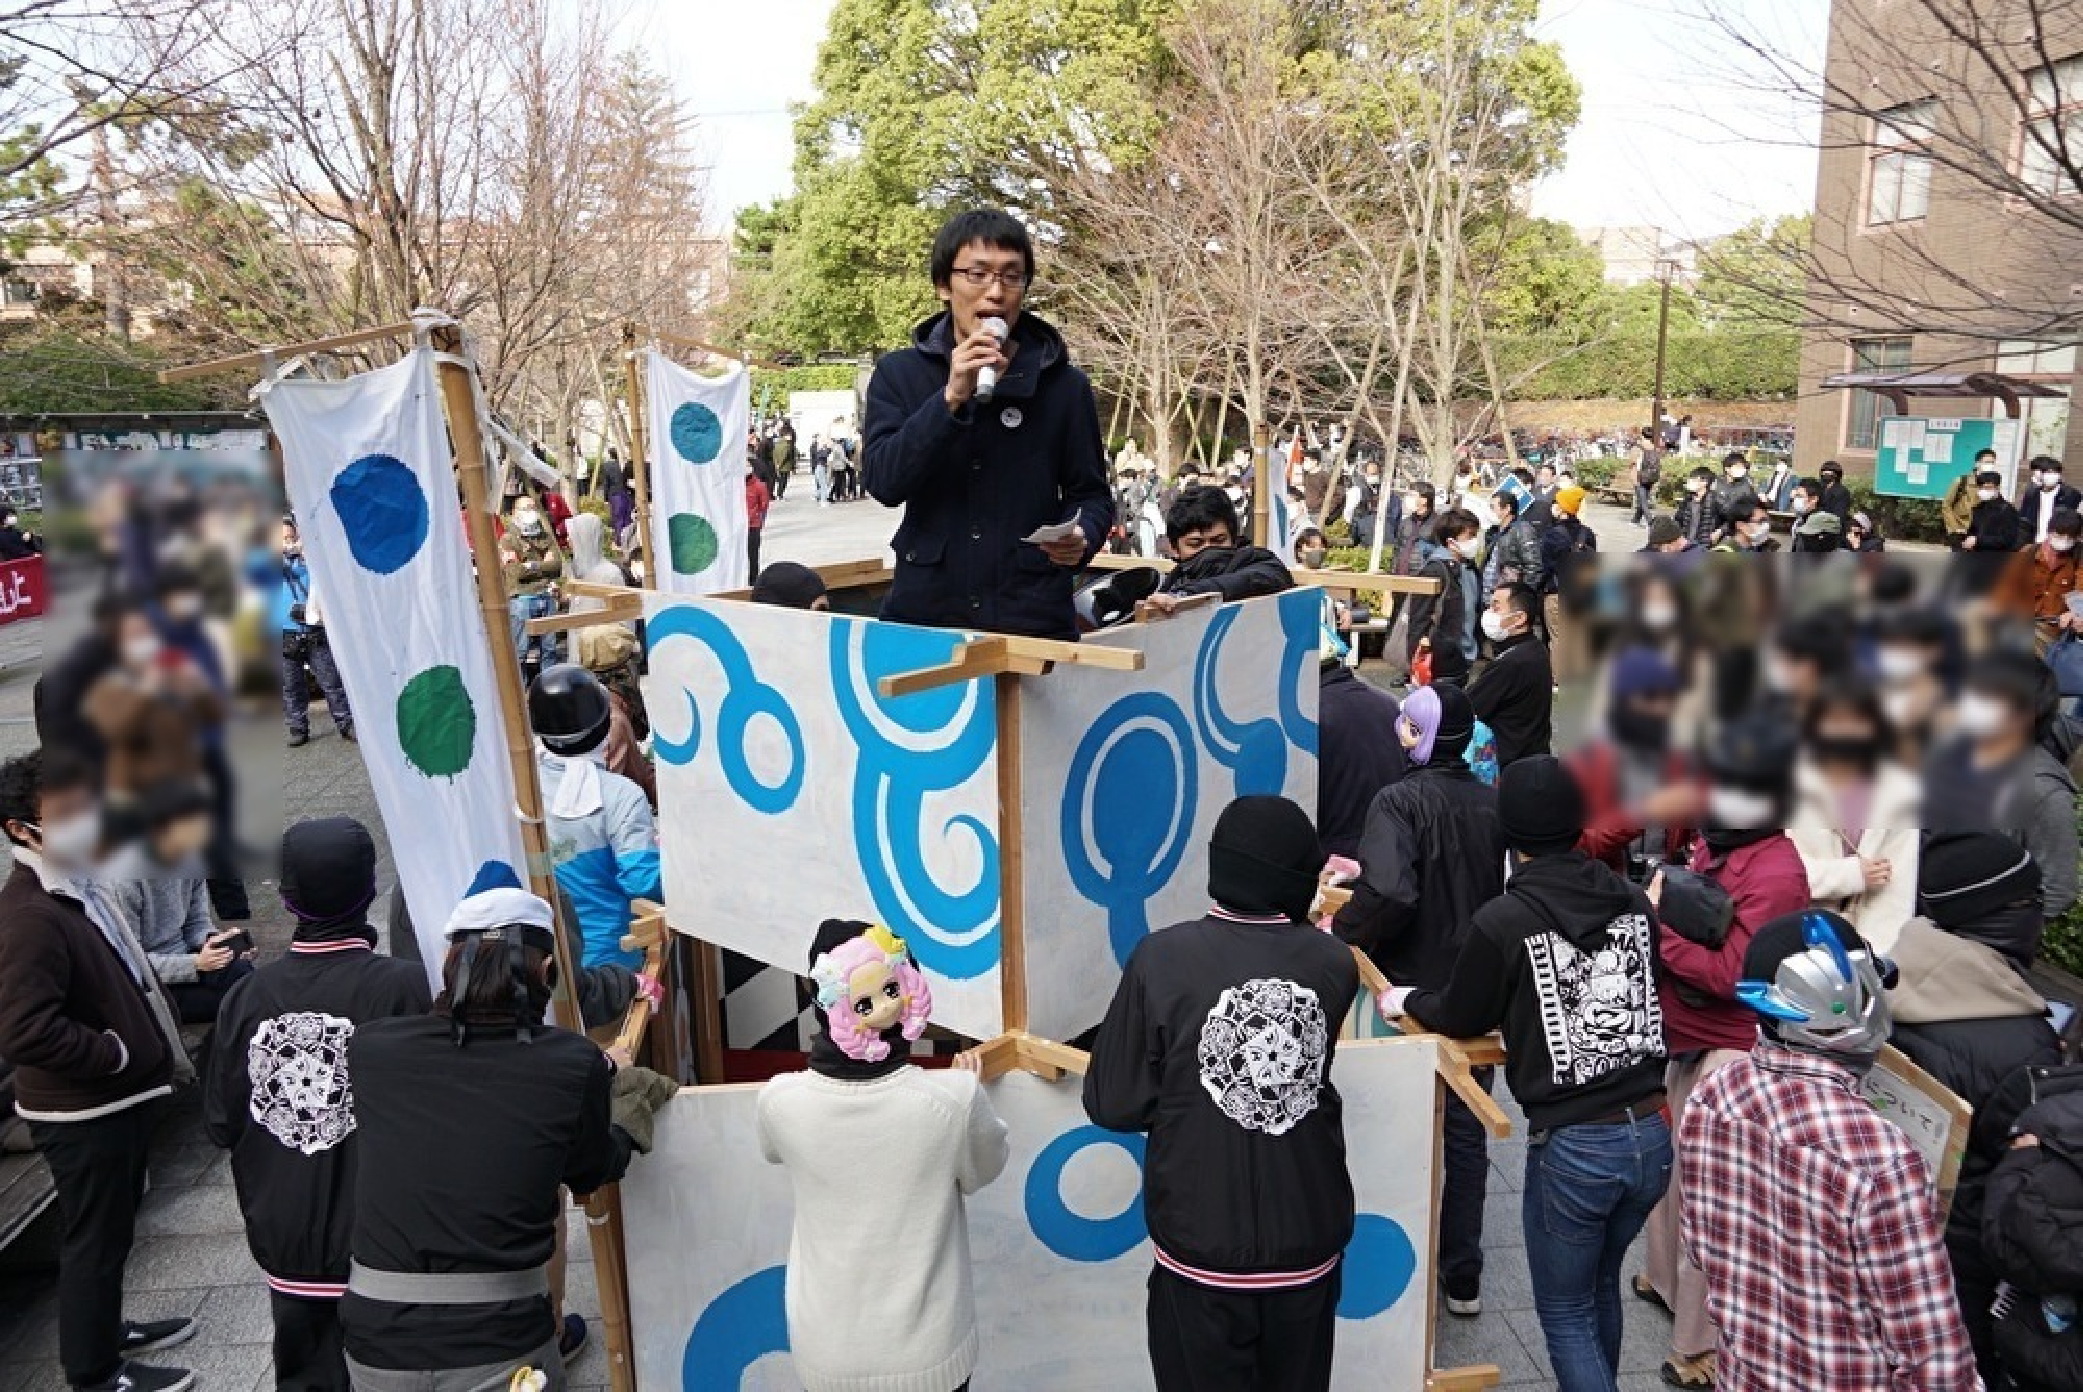
\includegraphics[width=18zw]{gazo/202112shukai.pdf}
    \captionsetup{labelformat=empty,labelsep=none}
    \caption{神輿に乗って演説する被処分者}
\end{wrapfigure}

 時計台占拠処分に向けた呼び出しが来た頃から全処対が主催して京大構内で集会が行われてきました。全処対主催で京大学生処分撤回・阻止 12 月緊急集会(通称「12 月集会」)が行われてきました。

 また、総長室突入を理由とした5学生への処分呼び出しが行われてからは熊野寮自治会主催での処分撤回・阻止集会も行ってきました。2024年7月に行った集会では、実際に呼び出しを受けている学生や大学当局によって言い渡されている学生含め熊野寮生が次々と発言に立ちました。当局は集会当日に大学職員を動員して集会への弾圧や出入り禁止の学生の排除を行ってきましたが、その場に集まった学生の力で出入り禁止処分を無効化して集会をやりきりました。文学部自治会学友会常任委員会や教員の先生方、他大学の学生団体からの賛同も得て広い陣形で集会を行うことができました。

 この集会には 2 つの意義があると思います。まず、多くの学生が集えば、当局がいくら集会を禁止しよう と集会できるのだと分かったことです。多くの学生が集えば表現の自由を守ることができるのです。逆に、表現の自由を守ろうという意志のもとにみんなが積極的に動かなければ、当局は簡単に学生の声を奪うことができたでしょう。権利や自由は当局によって与えられるものではなく、それを守ろうという不断の努力で私たち学生が作るものです。

 もう1つは、当局に対して、処分撤回・阻止で一致する学生の力を見せつけることができたことです。2019 年から多くの学生が不当な学生処分に対して声を上げ、集会や署名集めという形で行動を起こしてきたことで当局が下す処分の罪の重さ(停学期間の長さ等)が実際に軽くなっていたり、入試の像などの以前なら処分されていたことでも処分されなくなっていたりする現状があります。このように 多くの学生が集まれば集まるほど当局は処分を下しにくい状況、無期停学の解除や学生処分の撤回をせざるをえない状況に追い込まれるはずです。 


\subsection{お願い}
対処分戦略推進局はこれからも不当な処分攻撃に屈さず学生の権利を守っていけるよう活動を進めていきます。これを読んでいらっしゃる みなさんも、京大当局の動きに注意深く目を向けてください。当局が何か変なことをしたら、諦めるのではなく、立 ち上がってください。何をしたらいいのかわからなかったら、学部自治会や自治寮に顔を出してみてください。みな さんの力は学生の権利や自由を守ることに絶対に繋がります。w

\subsection{資料}


{\small
\begin{tcolorbox}[colback=white, colbacktitle=gray!30!white, coltitle=black, title=2024年9月25日付で京大生5名に下された懲戒処分に対する抗議声明,breakable]\index{せいめい@声明|(}

 2024年9月25日、2022年度熊野寮祭企画「総長室突入」に参加した熊野寮生5名に対し懲戒処分(うち1名に対し二ヶ月停学、4名に対し一ヶ月停学)が京都大学当局により下された。我々熊野寮自治会は、この懲戒処分を京都大学当局による学生の異議申し立て活動に対する不当な弾圧として糾弾する。以下に理由を述べる。

\noindent ○総長室突入の正当性\\
 2022年度寮祭企画「総長室突入」は学生との対話を拒み強権的に管理強化を進める京都大学当局に対する抗議の直接行動として、以下のような事項を要求した。
    
    \begin{enumerate}
        \item 保健診療所を廃止前と同水準で再開すること
        \item コロナ禍に乗じたサークル規制をやめること
        \item 11月祭に対する介入をやめること
        \item 学生自治寮への介入をやめること
        \item 京都大学立看板規程を撤廃すること
        \item 学生の活動に対する警察導入をやめること
        \item 学生懲戒規程を撤廃し、2016年から続く学生処分を撤回すること
        \item 学生の自由な活動を制限する一方的な授業改革(CAP制)をやめること
        \item 教職員に対する非正規職化や雇用雇止めをやめ、無期雇用転換を積極的に行うこと
        \item 各学生自治組織、並びに教職員組合からの団体交渉要求に誠実に応じ、合意に基づいた大学運営を行うこと
    \end{enumerate}
    
 以上10項目は学生や教職員の一般的利益として極めて正当な要求であり、事実企画当日には200名以上の学生が参加した。しかし、京都大学当局は事前に学生との対話抜きに一方的に告示を掲示して本企画を禁止し、学生窓口である厚生課へ行けと学生に指示してきたのみならず、最終的には警察を学生との合意なく入構させ学生を排除しようとした。

 しかし、熊野寮自治会含め学生はこれまでも継続的に厚生課窓口を通じ再三京都大学当局に対し改善を要求し続けており、それでも当局による管理強化は止まらなかったがために本企画のような抗議行動が起こされているのであって、この抗議活動に対してもこのような対応をとった京都大学当局は自身に対する批判に対し極めて不誠実に対応していると言わざるを得ない。

 そして、本懲戒処分は「学生を扇動」し「喧騒を激化」したことを理由に寮生5名を停学処分にしているが、これは当局が自身への批判を取り合わずただ「喧騒」として矮小化して鎮圧しようしていることの現れであり、今回の懲戒処分が当局が管理支配を強権的に進めていく上での政治的な弾圧として行われていることを示している。「総長室突入」が熊野寮自治会によって主催され多くの学生も参加した大規模な抗議行動であったにもかかわらず今回の五人のみに対し懲戒処分が科されているのは見せしめであり、学生の抗議行動を萎縮させるものである。

 「総長室突入」によって明るみに出たのは、抗議者に対し一方的に警察を導入したり懲戒処分したりする、学生と対話などする気のない現在の京都大学執行部の独裁的な態度だったのである。

\noindent ○停学処分の重さ・プロセス的な問題点\\
 また、今回かけられた停学処分は処分対象者の学生に多大な負担を強いる過酷なものであり、その決定に至るまでのプロセスにおいても問題がある。

 停学処分は対象となる学生の大学施設への出入りの一切を禁止するにも拘らず学費を徴収するため、事実上の罰金刑としての側面が存在する。また、今回下された懲戒処分は休学中の学生の休学状態を強制的に解除し、学費の支払い義務を発生させている。これは学生に決して安くはない学費を罰金として科すことにより京都大学当局に抗議する政治的な発言を封じようとするものであって、強く非難されるべきである。

 特に今回の懲戒処分は9月の末に通達されたため9月の末のわずかな日数に対しても一ヶ月分の学費支払い義務がきっかり発生しており、一ヶ月停学の場合は二ヶ月分の、二ヶ月停学の場合は三ヶ月分の学費の支払い義務が発生している。これによって京都大学当局は定められた停学期間で実際に構内に入ることのできない期間と学費の支払い義務を最大化しようとしており、全く姑息な工夫であると言わざるを得ない。

 また、過去の懲戒処分と同様に処分の決定に至るプロセスには問題が存在する。懲戒処分の対象となる学生は、聞き取り・弁明の機会の付与と称して京都大学当局から呼び出しを受けるが、この呼び出しは非公開・証拠の提示なし・弁護士含む第三者の同伴禁止などの不当な条件の下で行われる。これでは強権的かつ恣意的な証言の解釈が行われる、本人の意思に拘らず謝罪と反省を迫られるといった危険性がある。そしてなにより当局に対して弱い立場にある学生に対し、権力を持つ当局が一方的に処罰を押し付ける不均衡な構図自体非常に抑圧的で不当なものである。

 さらに、今回の懲戒処分に至るプロセスでは教授会による自治もまた無視されている。文学部から送付された陳述の機会を与えるとする文書において、処分者のうち一名に対しては当初譴責処分が検討されていると記載されていたが、実際にその学生に降ったのは一ヶ月の停学処分だった。ここから、文学部教授会が譴責処分で懲戒処分を上申したにも関わらず、総長により決定が覆され、教授会の判断よりも重い一ヶ月の停学処分が下されることになったと推測される。比較的軽いものになったとはいえ譴責処分を上申した文学部教授会の判断自体もまた批判されるべきものではあるが、学内自治の重要な構成員である教授会の議論の結果を無視して、さらに重い懲戒処分を独断的に下した京都大学当局の行動は教授会自治も踏み躙る極度の横暴であり、現在の当局の管理強化を一方的に進める姿勢をよく示す悪質なものである。

\noindent ○学生処分の本質的な不当性\\
 そもそも今回の懲戒処分に限らず、近年京都大学当局が行ってきた学生の行動に対する恣意的な処分は全て不当なものであり、学生全体への抑圧に他ならない。

 2016年以降、京都大学当局は熊野寮生を中心とした10名以上の学生に対し懲戒処分を行ってきたが、過去のこれらの処分も今回と同様の性質を持っている。過去にも京都大学当局は「業務妨害」を口実に、大学当局による管理強化・自治寮への攻撃に抗議した学生に対して、学生の言い分は一切顧みずに学生懲戒規程を恣意的に運用することによって懲戒処分を濫用してきた。その結果、学生は立て看板の一方的な規制や窓口における職員の不正な行為など、大学に疑義があっても、処分のおそれを前に萎縮させられ、理不尽を強いられ、大学の規制を受け入れざるを得ない状況に追い込まれてきた。こうして自治破壊が行われてきたのである。

 学生処分の問題は処分の対象となった学生だけには限定されない全学生にとっての問題である。特に、当局による廃寮化攻撃を含めた管理強化に抗議した学生が恣意的に処分されている以上、学生処分の問題は廃寮の問題と一体であり熊野寮自治会として看過できるものではない。また、学生処分は、数十年来、国策としての大学改革が学生の声を無視して一方的に進められ、全国の大学が「採算を取る」ことを要求される中で、多くの学生寮が廃寮に追い込まれ、学生の学びは管理され、生活が破壊されてきたことと一体の問題である。現在東京大学をはじめ、全国の大学で学費の値上げが問題となっている。これは大学改革政策における学生の生活破壊の最たるものであり、許されるものではない。京大当局も熊野寮や吉田寮との交渉を一方的に打ち切って廃寮化攻撃を行い、保健診療所も反対の声がある中で廃止を強行し、学内のガバナンス強化を要する国際研究卓越大学制度に率先して応募するなど大学改革を先頭で推し進める張本人として存在している。以上のような「改革」の障害となる学生に対して処分が行われてきたのである。

\noindent ○終わりに\\
 以上のように、本懲戒処分は管理強化を独断で進めようとする京都大学当局が抗議する学生に対し下した恣意的かつ過酷な攻撃に他ならないのであって、最も強い非難の言葉に値するものである。京都大学当局に対し我々熊野寮自治会は、当該5学生に対する懲戒処分を即時撤回し、「総長室突入」の要求10項目を受け入れることを求める。

熊野寮自治会

\vspace{5mm}
\noindent ▼今回の処分で用いられた規程\\
「京都大学学生懲戒規程」(平成29年2月28日 達示第103号全部改正)
(\url{http://www.kyoto-u.ac.jp/ja/about/organization/other/revision/documents/h28/t103-28.pdf})


\end{tcolorbox}
}

{\small
\begin{tcolorbox}[colback=white, colbacktitle=gray!30!white, coltitle=black, title=熊野寮生3名に対する無期停学処分の撤回を求める声明,breakable]\index{せいめい@声明|(}

    \begin{flushright}
    京都大学熊野寮自治会
    \end{flushright}
    \begin{flushleft}
    京都大学総長 山極壽一 殿 
    \end{flushleft}
    
    2019年9月10日付けで熊野寮生3名に対し無期停学処分が下されました。3名の行った行為はどれも「職員の行為を妨害」したものであり、京都大学通則第32条第1項に規定する「学生の本分を守らない」行為であるとされたためです。今回の処分について、以下の2点から抗議します。
    
    \begin{enumerate}
        \item 大学職員の行為の正当性を検証する場がない\\
         3名の行為・言動は、京都大学当局(以下、当局)の一方的な決定とそれを遂行する職員に対する抗議として行われました。
    
         学生との話し合いが一切行われない中で、当局の決定に従う職員は自らの職務を強硬的・暴力的に全うしようとし、学生がそれに抗議すれば否応なしに処分が下されます。
        正当性が検証されていない職務行為への妨害を理由とした処分は撤回されるべきです。
        
        \item そもそも懲戒規程の内容が恣意的に運用できるものである\\
         「京都大学学生懲戒規程」(平成29年2月28日 達示第103号全部改正)において懲戒の対象は「学生の本分を守らない者」とされ、さらにここでは「京都大学の諸規程又は命令に違反した者」がその具体的な項目の一つとして記されています。
    
         これによって当局の意思決定及びそれに従う職員の行為に反する学生を恣意的に処分することができるため、この規程による処分は撤回されるべきです。
    \end{enumerate}
    
     今回の処分は、立て看板規制や吉田寮現棟明け渡し訴訟、11月祭への介入など、当局が学生への規制・弾圧を推進する渦中で行われています。
    
     今後も当局が抗議する学生を処分することは容易に想像でき、その影響は現在だけでなく未来の京大生にまで及びます。大学の在り方を考える学生の権利・主体性が剥奪され、当局の意思決定に学生が反論し抗議することすらできない状況は、理性と言論の府たる大学において看過されるものではありません。
    
     熊野寮自治会は、寮生3名に対する無期停学処分の即時撤回、今後同様の形で学生を処分しないこと、そして今後の大学運営においては当事者である学生との話し合いを踏まえたうえで意思決定がなされることを求めます。
    
    \begin{flushright}
    2019年10月18日
    \end{flushright}
    
    \vspace{5mm}
    \noindent ▼京都大学による公式発表「学生の懲戒処分について」(2019年9月12日)\\
    (\url{http://www.kyoto-u.ac.jp/ja/about/events_news/office/kyoiku-suishin-gakusei-shien/kosei/news/2019/190912_1.html})
    
    \begin{quotation}
    本学は、文学部4回生1名、工学部4回生1名、総合人間学部4回生1名を、令和元年9月10日付けで、以下のとおり懲戒処分とすることを決定しました。
    \begin{enumerate}
        \item 文学部4回生1名を、京都大学通則第32条に定める「学生の本分を守らない者」として、令和元年9月10日付けで同通則第33条に定める停学(無期)処分とした。
        \item 工学部4回生1名を、京都大学通則第32条に定める「学生の本分を守らない者」として、令和元年9月10日付けで同通則第33条に定める停学(無期)処分とした。
        \item 総合人間学部4回生1名を、京都大学通則第32条に定める「学生の本分を守らない者」として、令和元年9月10日付けで同通則第33条に定める停学(無期)処分とした。
    \end{enumerate}
    
    \vspace{4mm}
    \noindent 処分理由
    \begin{enumerate}
        \item 文学部学生
        
         当該学生は、平成30年8月9日、オープンキャンパス初日に本部構内のクスノキ東側に設置された巨大工作物の一部に座り込み、当該工作物を撤去しようとする職員の行為を妨害するなどした。
    
         また、当該学生は、平成30年9月27日及び同年10月18日、教育推進・学生支援部棟2階の厚生課窓口及び廊下において、不審者を取り押さえようとする職員の行為を妨害するなどした。
    
         これらのことは、京都大学学生懲戒規程第3条第5号「前各号に準ずる不適切な行為を行った」に該当し、京都大学通則第32条第1項に規定する「学生の本分を守らない」行為である。
    
         よって、本学は、今回の行為の事実関係について調査を行い、慎重に審議した結果、当該学生を停学(無期)処分とすることとした。
        
        \item 工学部学生
        
         当該学生は、平成30年9月27日及び同年10月18日、教育推進・学生支援部棟2階の厚生課窓口及び廊下において、不審者を取り押さえようとする職員の行為を妨害するなどした。
    
         また、当該学生は、平成30年10月3日、吉田南構内において立入禁止対象者を構外へ連れ出そうとする職員の行為を妨害するなどした。
    
         これらのことは、京都大学学生懲戒規程第3条第5号「前各号に準ずる不適切な行為を行った」に該当し、京都大学通則第32条第1項に規定する「学生の本分を守らない」行為である。
    
         よって、本学は、今回の行為の事実関係について調査を行い、慎重に審議した結果、当該学生を停学(無期)処分とすることとした。
        
        \item 総合人間学部学生
    
         当該学生は、平成30年9月27日及び同年10月18日、教育推進・学生支援部棟2階の厚生課窓口及び廊下において、不審者を取り押さえようとする職員の行為を妨害するなどした。
    
         このことは、京都大学学生懲戒規程第3条第5号「前各号に準ずる不適切な行為を行った」に該当し、京都大学通則第32条第1項に規定する「学生の本分を守らない」行為である。
    
         よって、本学は、今回の行為の事実関係について調査を行い、慎重に審議した結果、当該学生を停学(無期)処分とすることとした。
        
    
    \end{enumerate}
    \end{quotation}
    
    \vspace{5mm}
    \noindent ▼今回の処分で用いられた規程\\
    「京都大学学生懲戒規程」(平成29年2月28日 達示第103号全部改正)
    \url{http://www.kyoto-u.ac.jp/ja/about/organization/other/revision/documents/h28/t103-28.pdf}
    
    \vspace{5mm}
    \noindent ▼補足\UTF{2160}.不審者取り押さえ時の状況
    
     3名に共通する処分理由である上記の「平成30年9月27日及び同年10月18日」の件は、熊野寮自治会による要求書提出の際に起こった出来事です。この際、2017年7月25日付で京都大学を放学処分となり、同年10月2日付で学外者として敷地内立入禁止とされた\UTF{9AD9}田暁典がストッキングとフルフェイスヘルメットを被り、水色のネズミの着ぐるみを装って提出行動に参加していました。10月18日の要求書提出後、職員約8名が彼を取り押さえ、顔を隠した素性不明の不審者として警察に引き渡し、不退去罪の現行犯として逮捕させました。\index{ようきゅうしょ@要求書}
    
     職員は退去しようとしていた\UTF{9AD9}田を大人数で取り押さえ、その手を踏みつけて流血させ、彼の退去を暴力的に阻止していました。この取り押さえ方に対し、寮生3名は職員と高田の間に割って入る、職員を高田から引き剥がすなどして、それを阻止しようとしました。
    
    \vspace{5mm}
    \noindent ▼補足\UTF{2161}.近年の京大内の管理強化について
    
     ここ数年、大学職員は顔を隠して活動する学生を取り締まっています。顔を隠した状態で学内に入ろうとする学生に対し素顔をさらせと職員が要求し、拒否した学生に対しては不審者と断定し学外に強制的に排除します。顔を確認することで個人を特定し、学内での行動を逐一監視したり、学部・研究室\index{けんきゅうしつ@研究室}の教授を通しての脅しをかけたりなど、あらゆる形で学生に対し圧力をかけています。オープンキャンパスなどで着ぐるみを着て学内で宣伝活動している学生もいますが、顔を隠している学生は無条件で全員排除というわけではなく、職員の一存で強制排除されるかどうかが決まります。
\end{tcolorbox}
}